%%%%%%%%%%%%%%%%%%%%%%%%%%%%%%%%%%%%%%%%%
% Beamer Presentation
% LaTeX Template
% Version 1.0 (10/11/12)
%
% This template has been downloaded from:
% http://www.LaTeXTemplates.com
%
% License:
% CC BY-NC-SA 3.0 (http://creativecommons.org/licenses/by-nc-sa/3.0/)
%
%%%%%%%%%%%%%%%%%%%%%%%%%%%%%%%%%%%%%%%%%

%----------------------------------------------------------------------------------------
%	PACKAGES AND THEMES
%----------------------------------------------------------------------------------------

\documentclass{beamer}

\mode<presentation> {

% The Beamer class comes with a number of default slide themes
% which change the colors and layouts of slides. Below this is a list
% of all the themes, uncomment each in turn to see what they look like.

%\usetheme{default}
%\usetheme{AnnArbor}
%\usetheme{Antibes}
%\usetheme{Bergen}
%\usetheme{Berkeley}
%\usetheme{Berlin}
%\usetheme{Boadilla}
%\usetheme{CambridgeUS}
%\usetheme{Copenhagen}
%\usetheme{Darmstadt}
%\usetheme{Dresden}
%\usetheme{Frankfurt}
%\usetheme{Goettingen}
%\usetheme{Hannover}
%\usetheme{Ilmenau}
%\usetheme{JuanLesPins}
%\usetheme{Luebeck}
\usetheme{Madrid}
%\usetheme{Malmoe}
%\usetheme{Marburg}
%\usetheme{Montpellier}
%\usetheme{PaloAlto}
%\usetheme{Pittsburgh}
%\usetheme{Rochester}
%\usetheme{Singapore}
%\usetheme{Szeged}
%\usetheme{Warsaw}

% As well as themes, the Beamer class has a number of color themes
% for any slide theme. Uncomment each of these in turn to see how it
% changes the colors of your current slide theme.

%\usecolortheme{albatross}
%\usecolortheme{beaver}
%\usecolortheme{beetle}
%\usecolortheme{crane}
%\usecolortheme{dolphin}
%\usecolortheme{dove}
%\usecolortheme{fly}
%\usecolortheme{lily}
%\usecolortheme{orchid}
%\usecolortheme{rose}
%\usecolortheme{seagull}
%\usecolortheme{seahorse}
%\usecolortheme{whale}
%\usecolortheme{wolverine}

%\setbeamertemplate{footline} % To remove the footer line in all slides uncomment this line
%\setbeamertemplate{footline}[page number] % To replace the footer line in all slides with a simple slide count uncomment this line

%\setbeamertemplate{navigation symbols}{} % To remove the navigation symbols from the bottom of all slides uncomment this line
}

\usepackage{graphicx} % Allows including images
\usepackage{booktabs} % Allows the use of \toprule, \midrule and \bottomrule in tables
\def\red#1{\textcolor{red}{#1}}
\def\blue#1{\textcolor{blue}{#1}}
\def\MWS{\textsf{MWS}\xspace}
\def\schemasearch{\textsf{SchemaSearch}\xspace}

\usepackage{amsfonts}
\usepackage{amsmath}
\usepackage{hyperref}
\usepackage{xspace}

\usepackage{bera}
\usepackage{xcolor}

\colorlet{punct}{red!60!black}
\definecolor{background}{HTML}{EEEEEE}
\definecolor{delim}{RGB}{20,105,176}
\colorlet{numb}{magenta!60!black}
\def\cS{\mathcal{S}}
\let\phi=\varphi\let\tilde=\widetilde
\def\mws{\textsf{MathWebSearch}\xspace}
\def\tms{\textsf{TeMaSearch}\xspace}
\def\els{\textsf{Elasticsearch}\xspace}
\def\cmml{\textsf{Content MathML}\xspace}
\def\pmml{\textsf{Presentation MathML}\xspace}
\def\xml{\textsf{XML}\xspace}
\def\xhtml{\textsf{XHTML}\xspace}
\def\xpath{\textsf{XPath}\xspace}
\def\arxiv{\textsf{arXiv}\xspace}
\def\latexml{\LaTeX{ML}\xspace}
\def\arxmliv{\textsf{ArXMLiv}\xspace}
\def\mathml{\textsf{MathML}\xspace}
\def\zblatt{\textsf{Zentralblatt}\xspace}
\def\latex{\LaTeX\xspace}
\def\tex{\TeX\xspace}

%----------------------------------------------------------------------------------------
%	TITLE PAGE
%----------------------------------------------------------------------------------------

\title[Math Faceted Search]{\huge{Faceted Search in Mathematics}} 
\author[Hambasan Radu]{Hambasan Radu\\ \and Supervisor: Michael Kohlhase} 

\institute[JUB]
{
    \textit{r.hambasan@jacobs-university.de}\\
    \vspace{9mm}
    
\includegraphics[scale=0.4]{img/jub-logo}\\
    Bachelor Thesis in Computer Science
}
\date{\today} % Date, can be changed to a custom date

\begin{document}

\begin{frame}
\titlepage % Print the title page as the first slide
\end{frame}

\begin{frame}
\frametitle{Overview}
\tableofcontents
\end{frame}

\section{Introduction} 
%------------------------------------------------
\begin{frame}
\frametitle{Why math search?}
\begin{itemize}
    \item\visible<2->{Textual search engines cannot index math.}
\end{itemize}
\vspace{3mm}
\visible<3->{
    \begin{figure}
        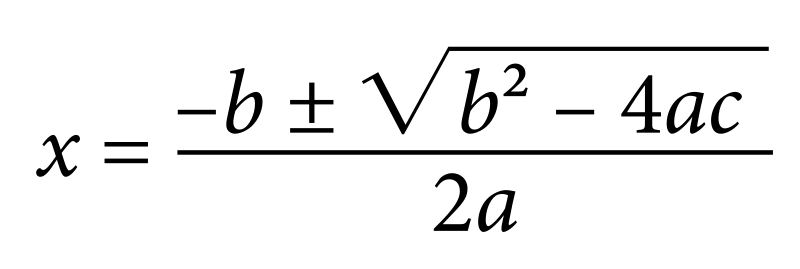
\includegraphics[scale=0.3]{img/math_example}
        \caption{Typical Formula}
    \end{figure}
}
\end{frame}
%------------------------------------------------
\begin{frame}
\frametitle{Why faceted search?}
\begin{itemize}
    \item It's important to allow the user to refine the query.
\end{itemize}
\end{frame}
%------------------------------------------------
\begin{frame}
    \begin{figure}
        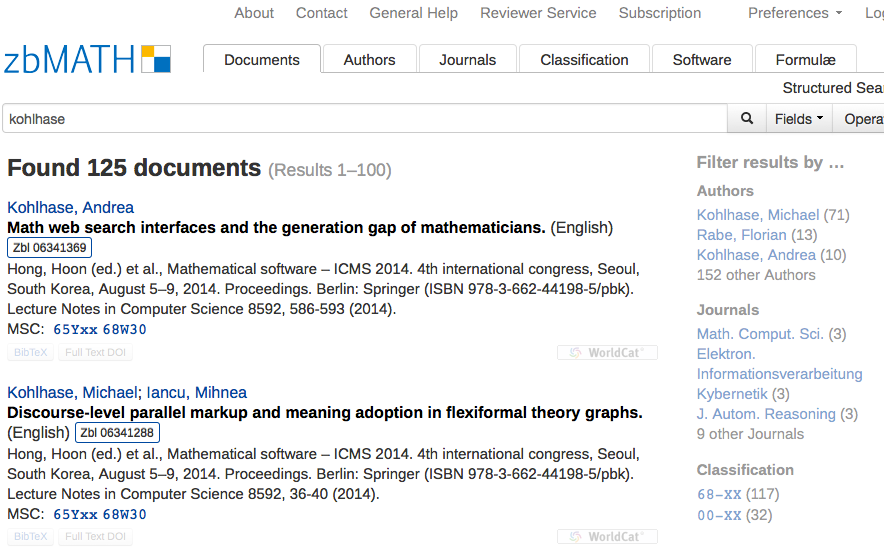
\includegraphics[scale=0.40]{img/faceted-search}
        \caption{Faceted Search Example}
    \end{figure}
\end{frame}
%------------------------------------------------
\begin{frame}
\frametitle{Formula Facets}
\begin{itemize}
    \item\visible<2->{Another dimension for refining a query.}
    \item\visible<3->{Based on the \textbf{meaning} of formulae.}
    \item\visible<4->{Can be described by \textit{formula schemata}.}
\end{itemize}
\vspace{3mm}
\visible<5->{
    \begin{figure}
        \begin{tabular}{l}
            $\int_{\red{M}}{\red\Phi(d_p\red{f}) dvol}$\\[1ex]
            $\lambda{\red{X}}.h(H^1\red{X})\cdots{H^n\red{X}}$\\[1ex]
            $\frac{\red\Gamma\vdash\red{A}\gg\red\alpha}{\red{D}}$
        \end{tabular}\vspace*{-.5em}
        \caption{Formula Schemata as Formula Facets}
    \end{figure}
}
\end{frame}
%------------------------------------------------

\section{Preliminaries}
\begin{frame}
\frametitle{Preliminaries}
\begin{itemize}
    \item{MathWebSearch (MWS)}
    \item{Elasticsearch (ES)}
\end{itemize}
\end{frame}
%------------------------------------------------
\subsection{MathWebSearch}
\begin{frame}
\frametitle{MathWebSearch}
\begin{itemize}
    \item\visible<2->{content-based search engine for math}
    \item\visible<3->{indexes \textsf{MathML} using Substitution Tree Indexing}
    \item\visible<4->{formulae are inserted in the index according to their DFS
        traversal}
    \item\visible<5->{the index nodes are unique integers corresponding to
        \textsf{MathML} elements.}
    \item\visible<6->{a \textsf{FormulaID} is assigned to each formula.}
\end{itemize}
\end{frame}
%------------------------------------------------
\begin{frame}
    \frametitle{Example}
\begin{itemize}
    \item Formula: $\frac{2}{x+3}$
\end{itemize}
\visible<2->{
    \begin{figure}
        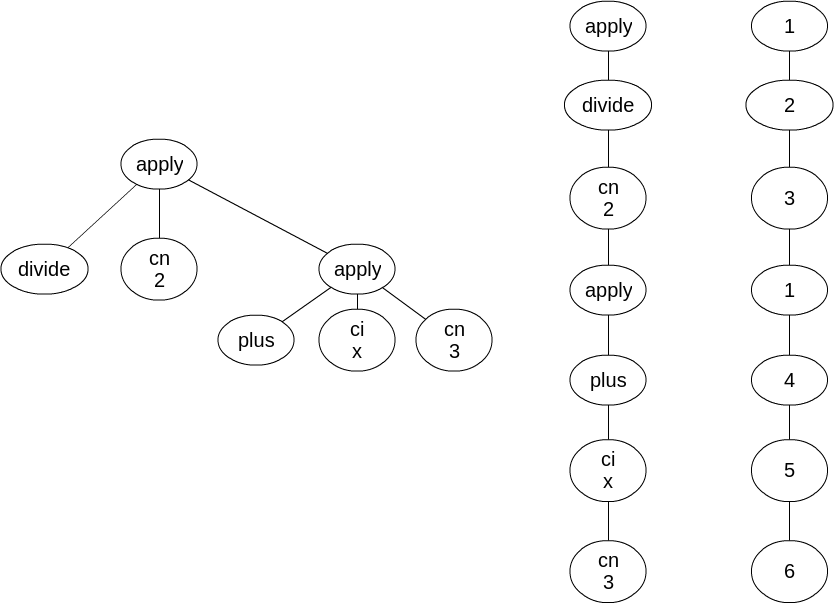
\includegraphics[scale=0.27]{img/mws_index_explained}
        \caption{MWS Index}
    \end{figure}
}
\end{frame}
%------------------------------------------------

\subsection{Elasticsearch}
\begin{frame}
\frametitle{Elasticsearch}
\begin{itemize}
    \item\visible<1->{powerful \& efficient text search and analytics engine}
    \item\visible<2->{built on top of Lucene}
    \item\visible<3->{massively scalable \& fault tolerant }
    \item\visible<4->{provides faceted search features (aggregations)}
    \item\visible<5->{We can use it to run aggregations on formulae.}
\end{itemize}
\end{frame}

%------------------------------------------------
\section{The Formula Schematizer}
\subsection{Purpose}
\begin{frame}
\frametitle{Purpose}
\begin{figure}
    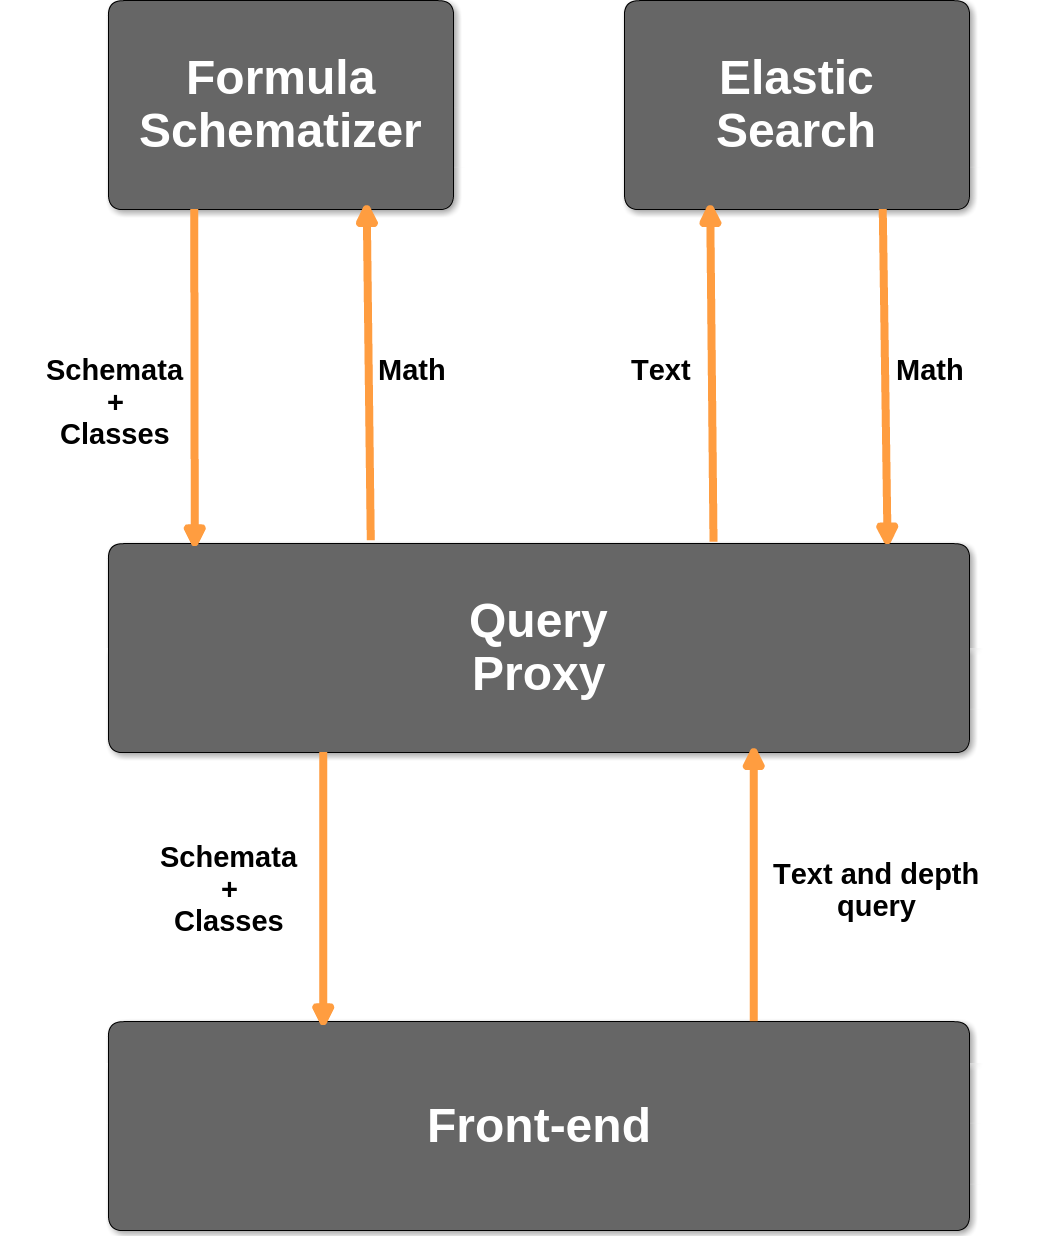
\includegraphics[scale=0.12]{img/SchemaArchitecture}
    \caption{FS Engine Architecture}
\end{figure}
\end{frame}
%------------------------------------------------
\subsection{Working Principle}
\begin{frame}
\frametitle{Working Principle}
\begin{itemize}
    \item\visible<1->{Idea: use the index to generate similar schemata}
\end{itemize}
\vspace{3mm}
\visible<2->{
    \begin{figure}
        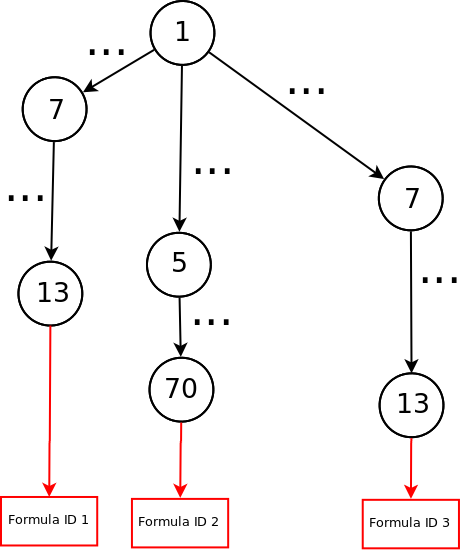
\includegraphics[scale=0.17]{img/naive_index}
        \caption{Simplified Index at depth 1}
    \end{figure}
}

\end{frame}
%------------------------------------------------
\begin{frame}
\frametitle{Working Principle}
\begin{enumerate}
    \item[1.]\visible<2->{Obtain \textsf{MathML} representation of formulae set.}
    \item[2.]\visible<3->{Create the table of signatures using a cutoff heuristic.}
\end{enumerate}
\visible<3->{
    \begin{figure}
        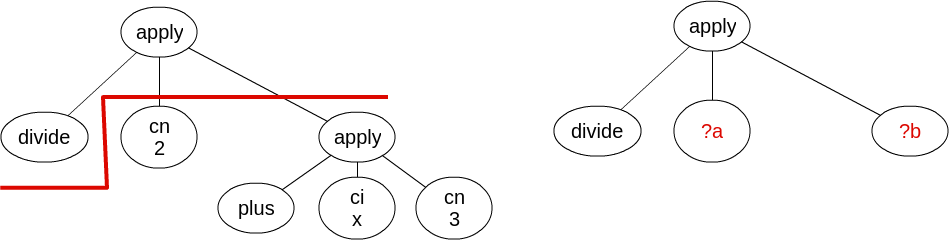
\includegraphics[scale=0.32]{img/cutoff_dynamic}
        \caption{Dynamic Cutoff}
    \end{figure}
}
\end{frame}
%----------------------------------------
\begin{frame}
\begin{enumerate}
    \item[3.]\visible<2->{Process the table.}
    \item[4.]\visible<3->{Generate \cmml schemata.}
    \item[5.]\visible<4->{Create \pmml schemata (\textbf{presentation by
        replacement}).}
\end{enumerate}

\visible<4->{
    \begin{figure}
        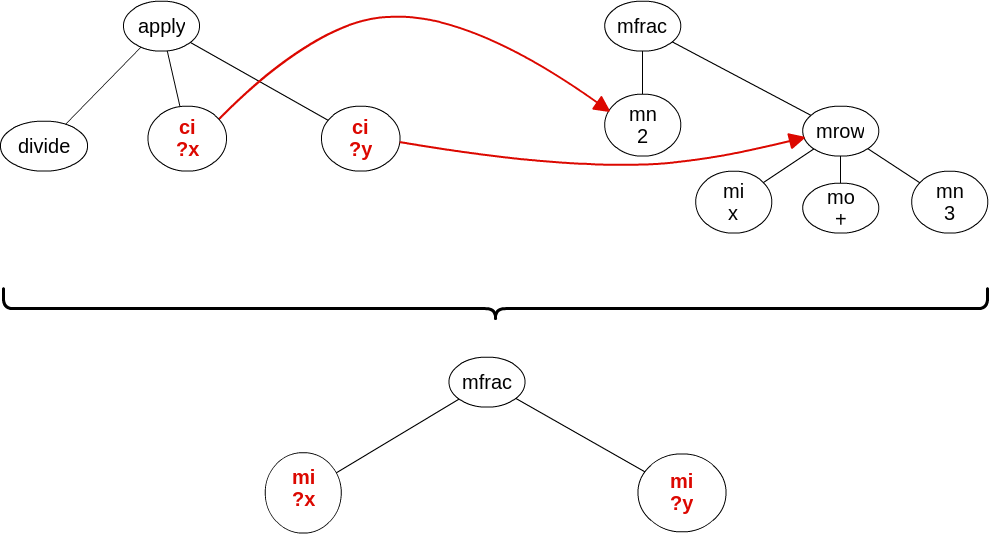
\includegraphics[scale=0.25]{img/replacement_pres}
        % Doesn't fit in page properly :(
        %\caption{Presentation by replacement.}
    \end{figure}
}
\end{frame}
%------------------------------------------------
\section{Evaluation of Results}
%------------------------------------------------
\subsection{SchemaSearch}
\begin{frame}
\frametitle{SchemaSearch}
\begin{itemize}
    \item\visible<2->{Text-only search}
    \item\visible<3->{Ideal for exploring a corpus}
    \item\visible<4->{It returns schemata \& formula classes}
    \item\visible<5->{Used mainly to showcase to \textsf{Schematizer}}
\end{itemize}
\end{frame}
%------------------------------------------------
\begin{frame}
    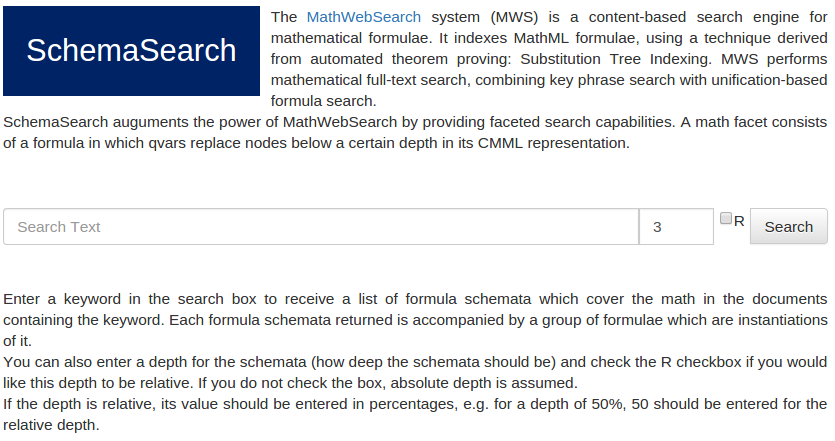
\includegraphics[width=\textwidth]{img/frontend_schema}
\end{frame}
%------------------------------------------------
\begin{frame}
    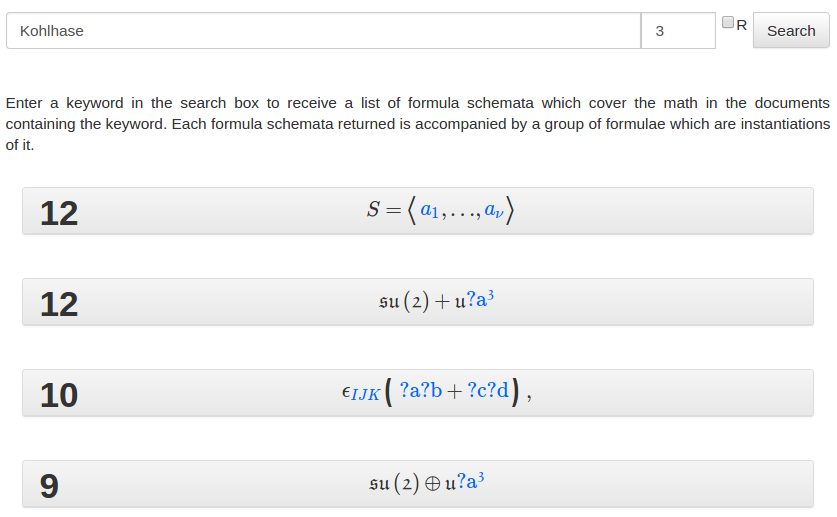
\includegraphics[width=\textwidth]{img/schemataGroup}
\end{frame}
%------------------------------------------------
\begin{frame}
    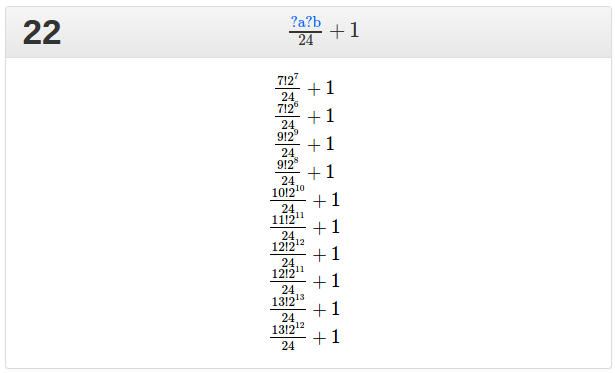
\includegraphics[width=\textwidth]{img/schemaInstGood}
\end{frame}
%------------------------------------------------
\begin{frame}
    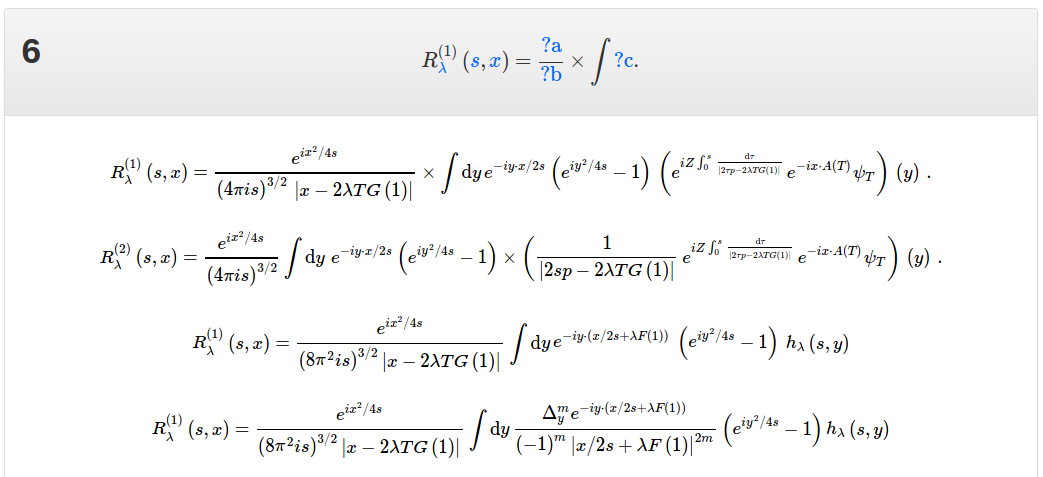
\includegraphics[width=\textwidth]{img/schemaInstGood3}
\end{frame}
%------------------------------------------------
\subsection{TeMa v2}
\begin{frame}
\frametitle{TeMa v2}
\begin{itemize}
    \item\visible<2->{Text and formula search}
    \item\visible<3->{Schemata filter query results}
    \item\visible<4->{Main demo for faceted search}
\end{itemize}
\end{frame}
%------------------------------------------------
\begin{frame}
    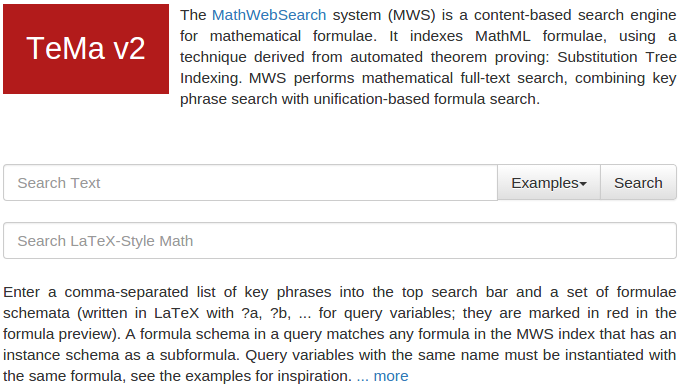
\includegraphics[width=\textwidth]{img/frontend_temaV2}
\end{frame}
%------------------------------------------------
\begin{center}
    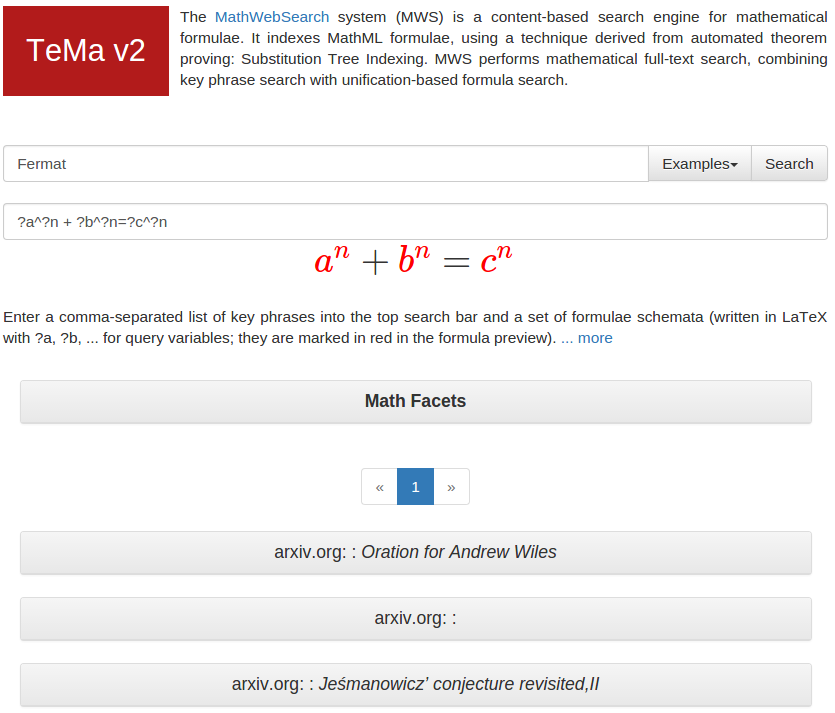
\includegraphics[height=0.9\textheight]{img/temaV2_results}
\end{center}
%------------------------------------------------
\begin{center}
    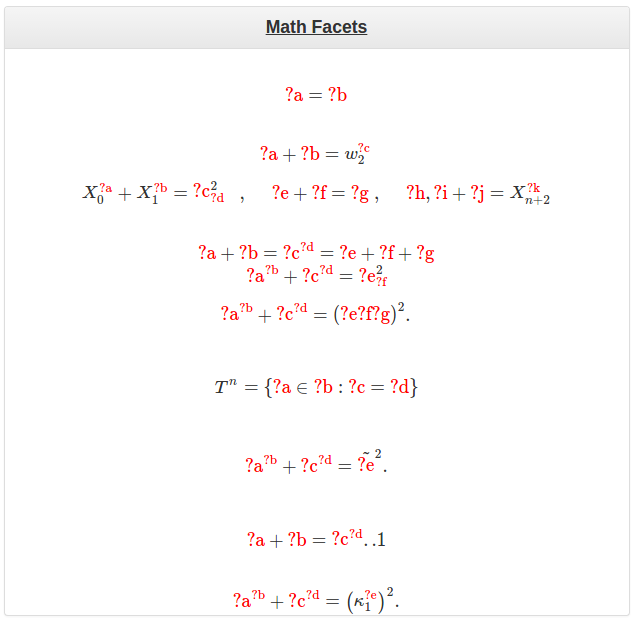
\includegraphics[height=0.9\textheight]{img/temaV2_facets}
\end{center}
%------------------------------------------------
\section{Future Work}
\begin{frame}
\frametitle{Future Work}
\begin{itemize}
    \item Similarity Search
    \item Improving NNexus
\end{itemize}
\end{frame}
%------------------------------------------------
\begin{frame}
    \frametitle{Demos}
    \begin{itemize}
        \item \textbf{SchemaSearch}:\\
            \textsf{http://jupiter.eecs.jacobs-university.de/schema}
        \item \textbf{TeMa v2}:\\
            \textsf{http://jupiter.eecs.jacobs-university.de/temaV2}
    \end{itemize}
\end{frame}
%------------------------------------------------
\section{Discussion}
\begin{frame}
\tableofcontents
\end{frame}
%------------------------------------------------

\end{document} 
